% \subsubsection{Accuracy}

% Based on the quantitative trends observed in Figures~\ref{fig:yolomobilenetv4} and~\ref{fig:code_generation}, the original YOLOv11n model achieves slightly higher detection accuracy compared to the YOLOv11n-MobileNetV4 variant. Specifically, the original model attains marginally better precision, recall, and mean Average Precision across the evaluated metrics.

% From the mAP@50 curves, the original YOLOv11n model achieves an improvement of approximately 10--15\% compared to the MobileNetV4-based model. A similar performance gap is observed for mAP@50--95, where the original architecture demonstrates around 10--15\% higher accuracy under stricter localization thresholds. These differences indicate that the original backbone provides stronger feature representation capability, particularly for precise object localization.

% Nevertheless, the overall performance gap remains relatively small. The YOLO-MobileNetV4 model preserves more than 95\% of the detection accuracy achieved by the original YOLOv11n while significantly reducing model complexity. Precision and recall curves further confirm that both models exhibit comparable convergence behavior, with the MobileNetV4 variant showing slightly lower but stable accuracy throughout training.

% These results highlight a clear trade off between accuracy and efficiency. While the original YOLOv11n model offers slightly superior detection accuracy, the YOLO-MobileNetV4 configuration provides a more balanced solution by achieving competitive accuracy with reduced computational cost. This balance makes the MobileNetV4-based model particularly suitable for deployment in edge oriented and resource constrained environments where efficiency is a primary concern.


% \begin{figure}[H]
%     \centering
%     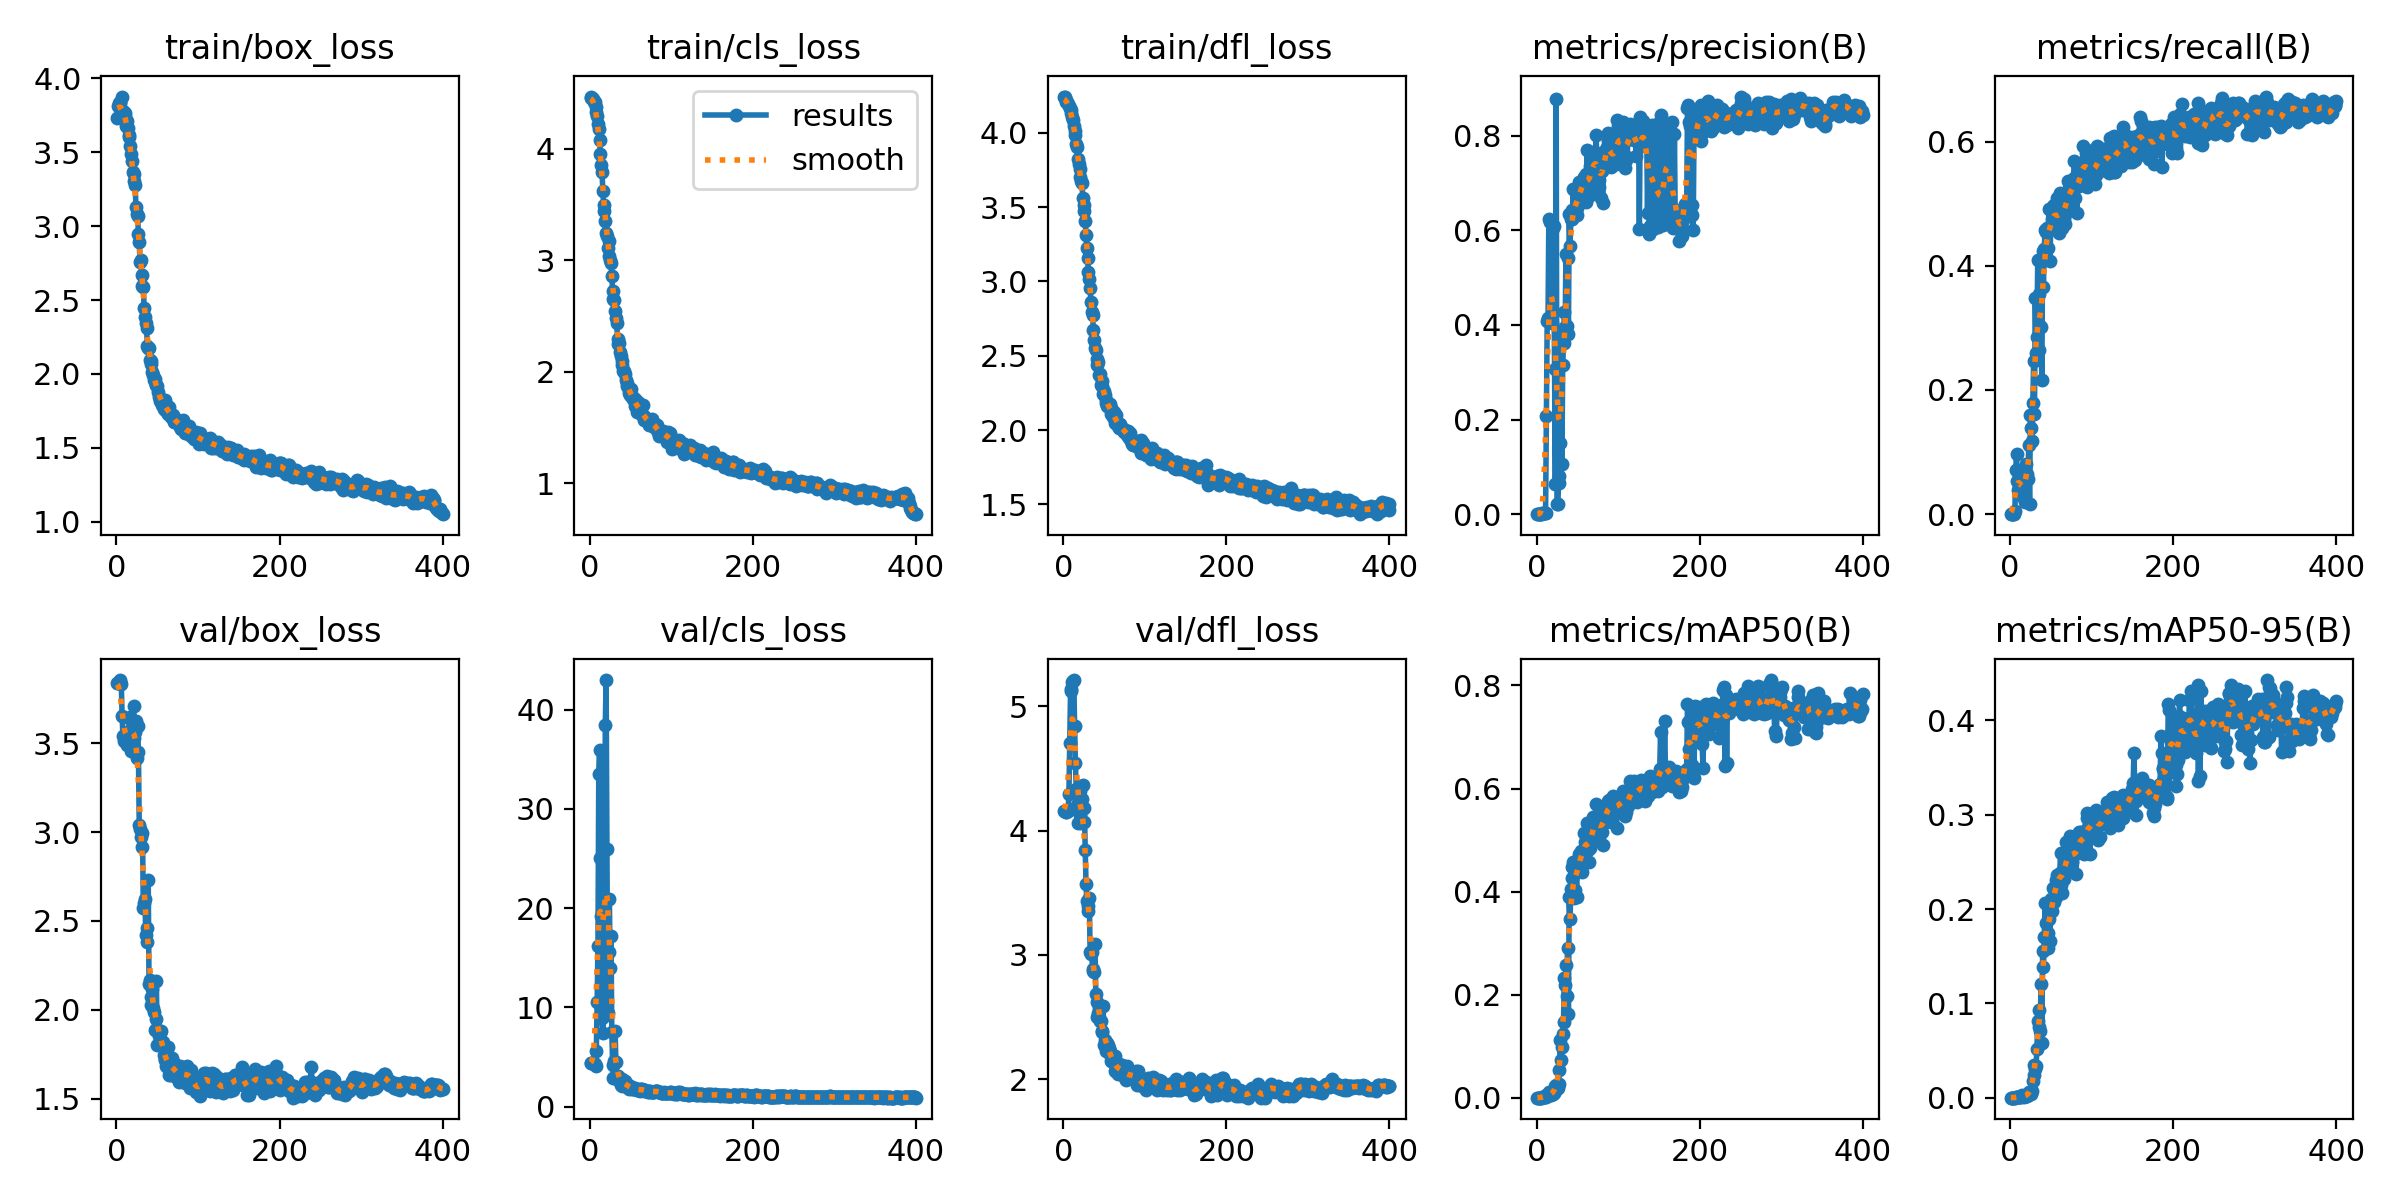
\includegraphics[width=0.75\textwidth]{Images/chap3/yolo/yolomobilenetv4.png}
%     \vspace{0.5cm}
%     \caption{The accuracy of Yolov11n-MobileNetV4}
%     \label{fig:yolomobilenetv4}
% \end{figure}

% \begin{figure}[H]
%     \centering
%     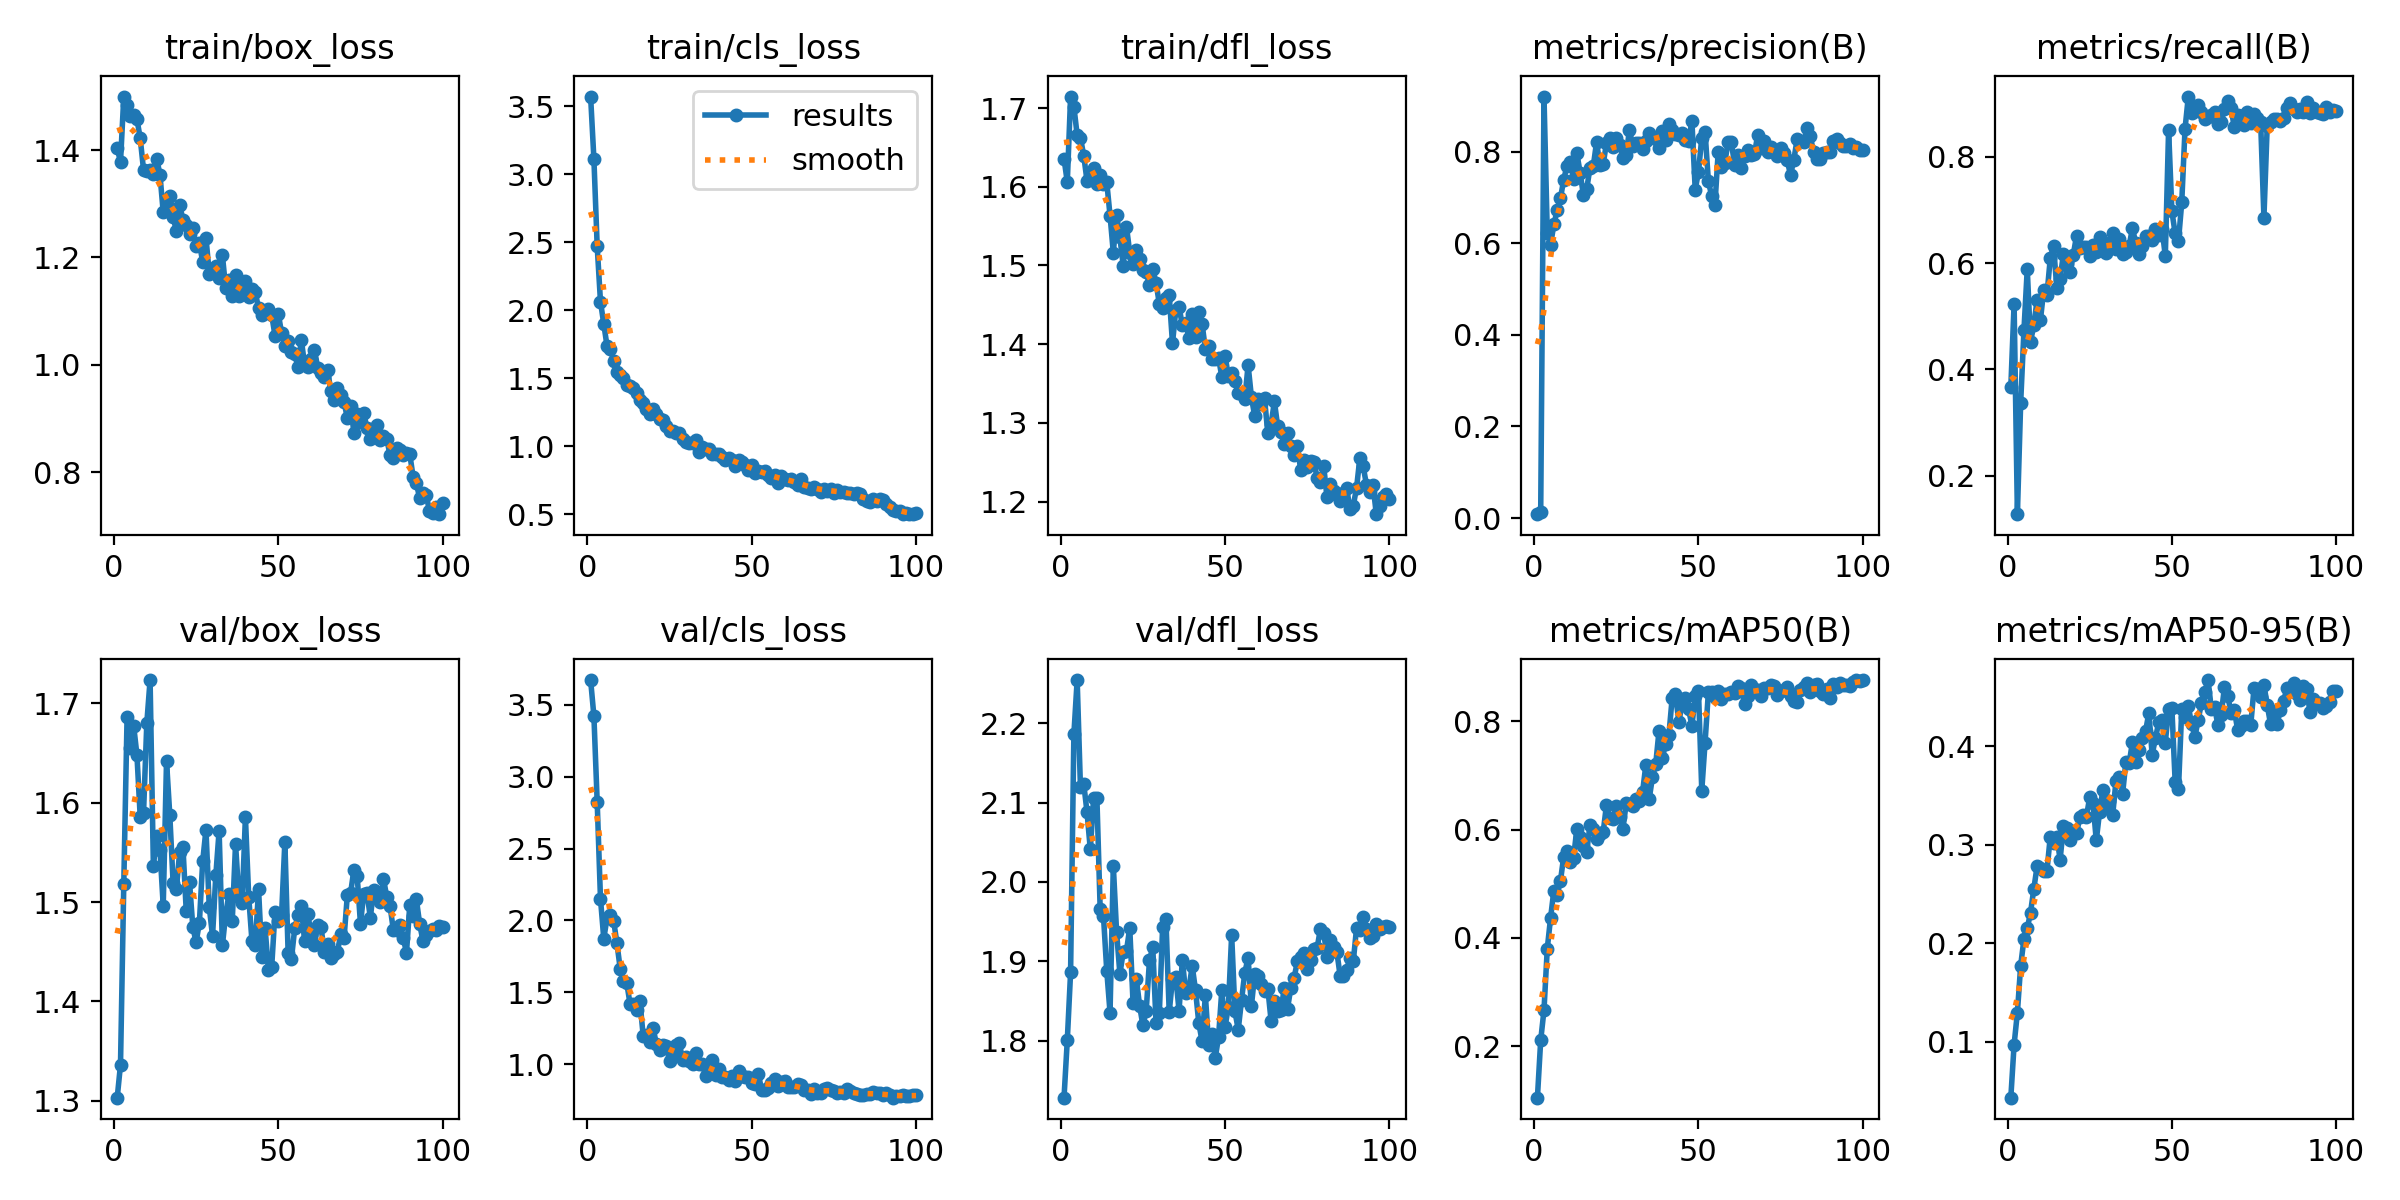
\includegraphics[width=0.75\textwidth]{Images/chap3/yolo/original.png}
%     \vspace{0.5cm}
%     \caption{The accuracy of original Yolov11n}
%     \label{fig:yolo11n}
% \end{figure}

% \subsubsection{Inference Speed}

% Inference speed is a key requirement for real time deployment on resource constrained platforms such as Raspberry Pi. According to the official Ultralytics benchmark, the original YOLO model converted to TensorFlow Lite requires more than 400\,ms per inference on Raspberry Pi class hardware when executed on CPU\footnote{Detailed benchmarking results for YOLO models on Raspberry Pi are reported by Ultralytics at \url{https://docs.ultralytics.com/vi/guides/raspberry-pi/\#detailed-comparison-table}.}. This latency corresponds to a processing rate of approximately 2--3 frames per second, which is insufficient for real time applications.

% In contrast, experimental results obtained in this work show that the YOLO-MobileNetV4 model achieves an average inference time of 30--40\,ms per frame after conversion to the TFLite format. This corresponds to an effective processing speed of approximately 25--33 frames per second. Compared to the original YOLO TFLite model, the MobileNetV4 based configuration reduces inference latency by approximately 360--370\,ms per frame.

% In relative terms, this represents a speed improvement of about 10--13 times. Equivalently, the inference time is reduced by approximately 90--92\% compared to the original YOLO TFLite implementation. Such a significant reduction enables near real time performance on CPU only embedded devices.

% The observed speedup is primarily attributed to the lightweight architecture of the MobileNetV4 backbone, which substantially reduces the number of parameters and floating point operations. As a result, the YOLO-MobileNetV4 model achieves a much more favorable balance between detection accuracy and inference speed, making it well suited for real time edge deployment on Raspberry Pi platforms.

% \begin{figure}[H]
%     \centering
%     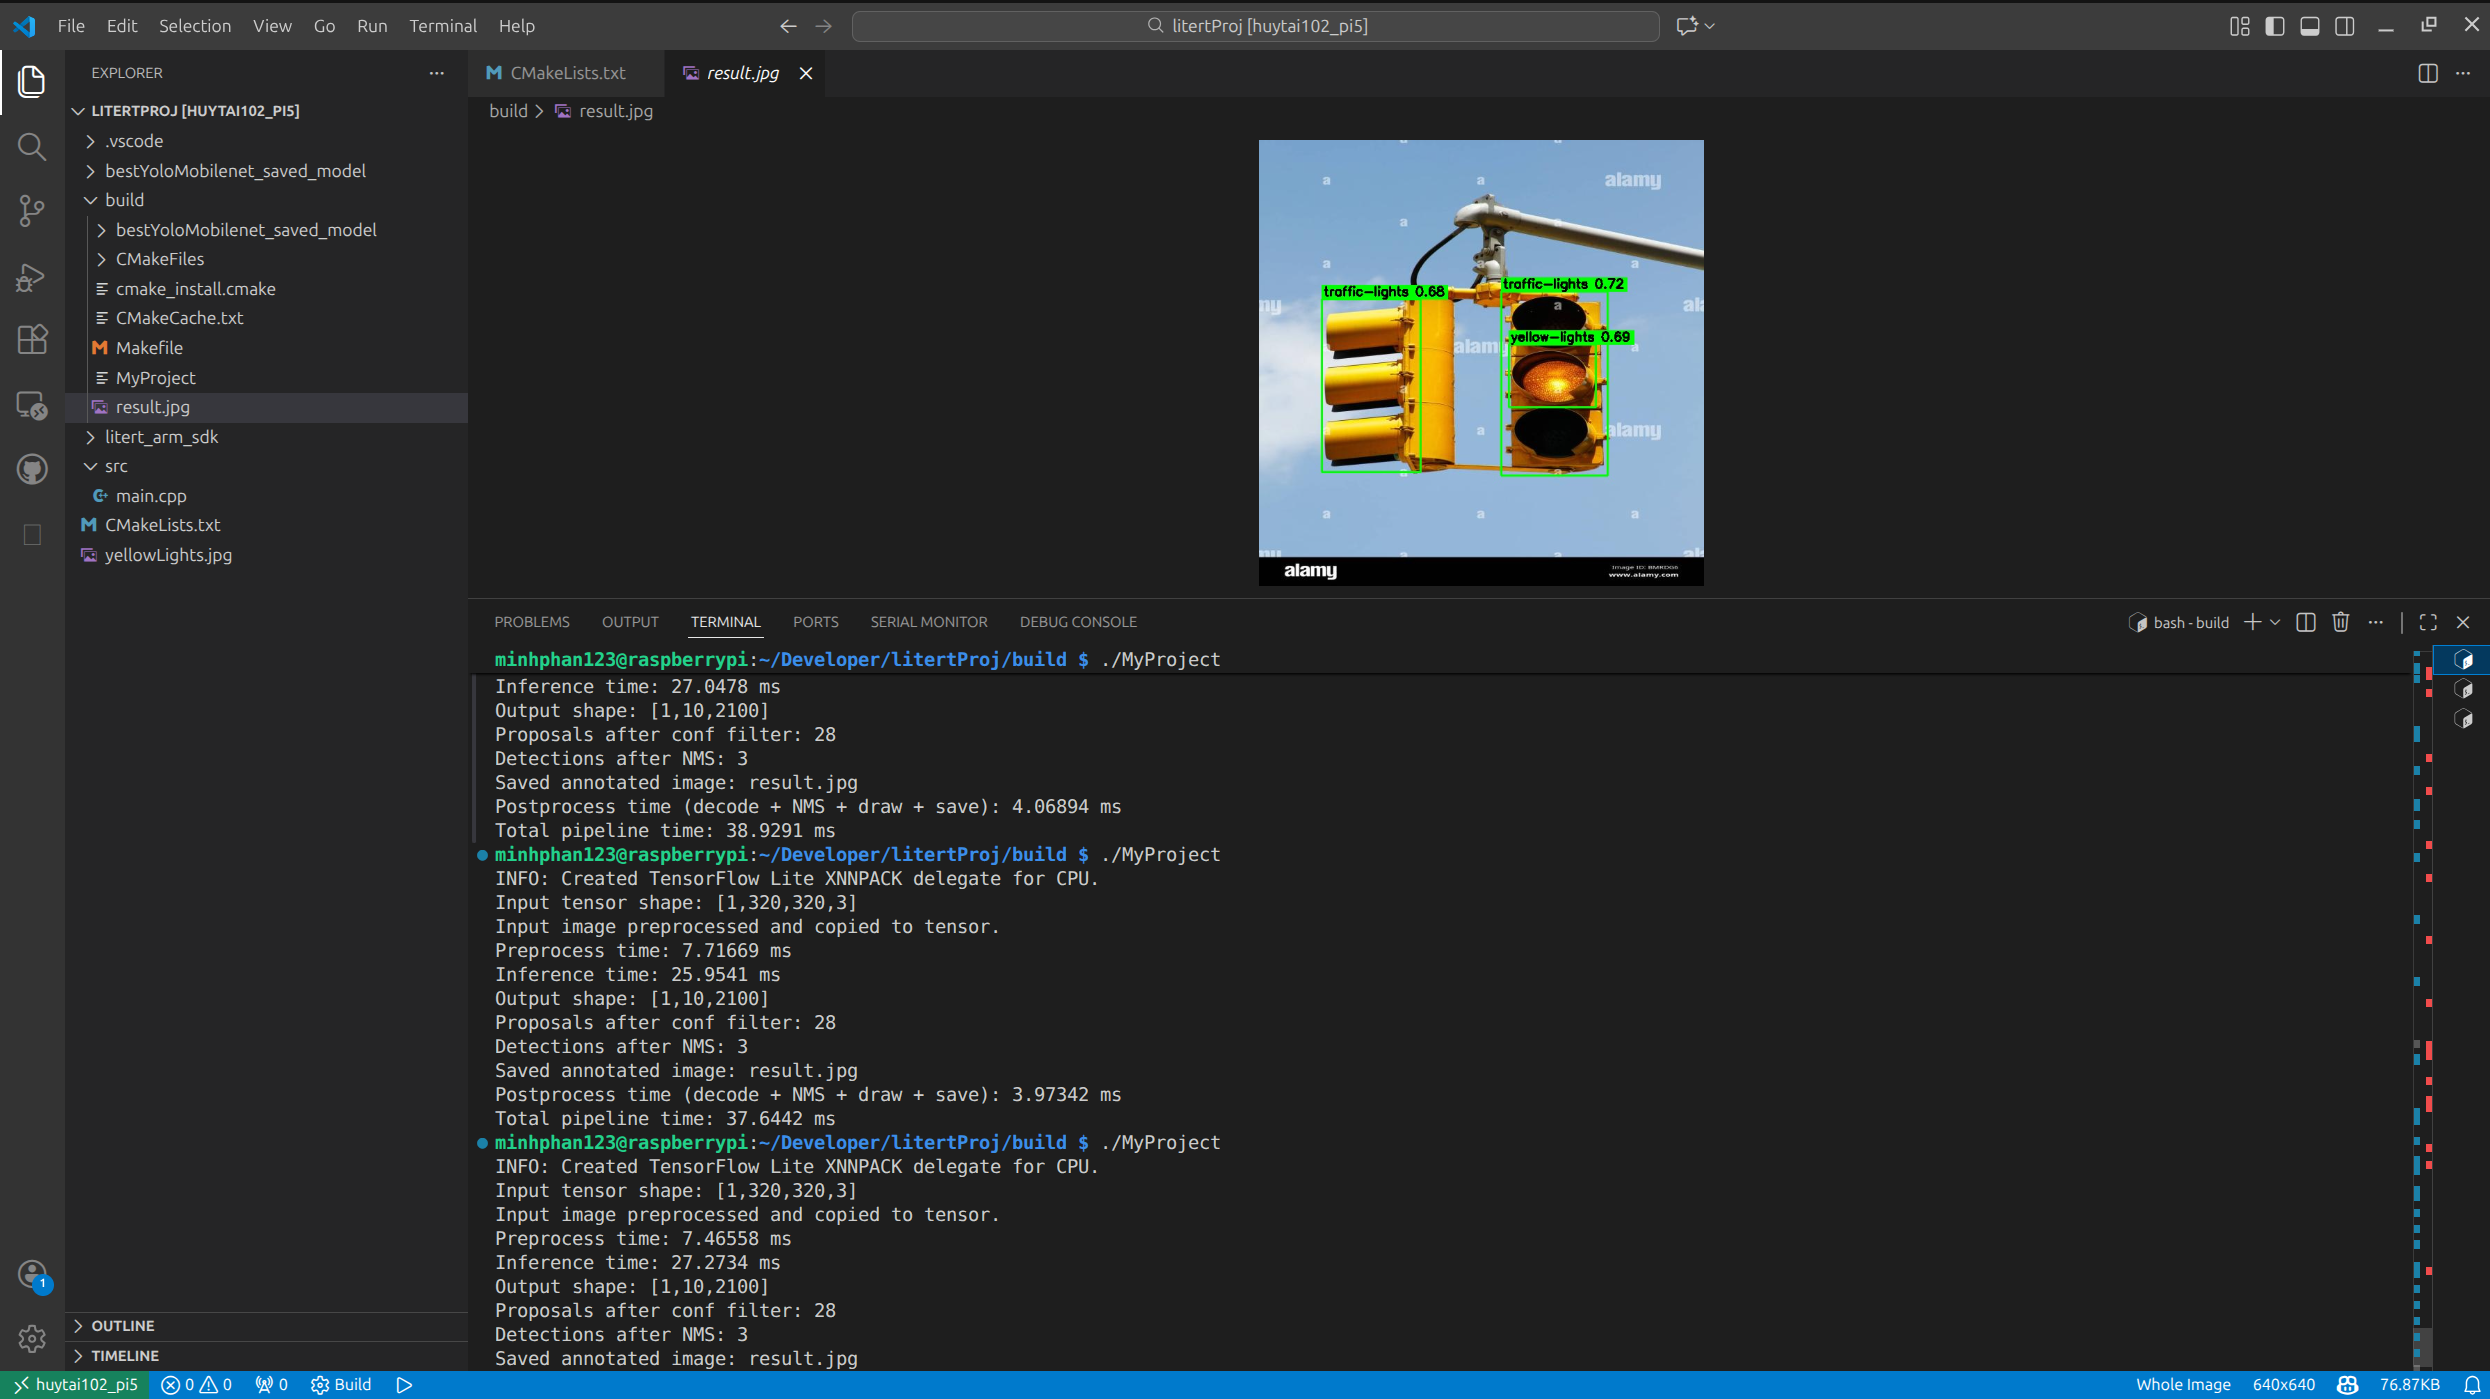
\includegraphics[width=0.75\textwidth]{Images/chap3/yolo/inference_speed.png}
%     \vspace{0.5cm}
%     \caption{The inference time of Yolovv11n-MobileNetV4 model}
%     \label{fig:infer_time_yolo11n_mobilenetv4}
% \end{figure}


% \begin{table}[H]
% \centering
% \label{tab:tradeoff_yolo_models}
% \begin{tabular}{|l|c|c|}
% \hline
% \textbf{Metric} & \textbf{YOLOv11n (Original)} & \textbf{YOLOv11n-MobileNetV4} \\
% \hline
% Backbone & CSP-based YOLO backbone & MobileNetV4 (lightweight) \\
% \hline
% mAP@50 & Higher ($\approx$ +10--15\%) & Slightly lower \\
% \hline
% mAP@50--95 & Higher ($\approx$ +10--15\%) & Slightly lower \\
% \hline
% Precision / Recall & Marginally higher & Comparable and stable \\
% \hline
% Inference time (TFLite, CPU) & $>$400 ms & 30--40 ms \\
% \hline
% Throughput (FPS) & 2--3 FPS & 25--33 FPS \\
% \hline
% Speedup factor & 1$\times$ (baseline) & $\approx$10--13$\times$ faster \\
% \hline
% Inference time reduction & -- & $\approx$90--92\% \\
% \hline
% Model complexity & Higher & Significantly reduced \\
% \hline
% Suitability for edge deployment & Limited & Highly suitable \\
% \hline
% \textbf{Overall trade-off} & Higher accuracy & Better accuracy--speed balance \\
% \hline
% \end{tabular}
% \caption{Trade-off comparison between YOLOv11n and YOLOv11n-MobileNetV4}
% \end{table}

\subsection{Evaluation between Models}

To validate the architectural modifications introduced by the MobileNetV4 backbone replacement, a systematic benchmark was conducted comparing the original YOLO26n model against the proposed YOLO26n-MobileNetV4 variant. 

Both models were evaluated on the same TrafficLightV5 validation set under identical conditions: $416 \times 416$ input resolution, INT8 TFLite quantisation, batch size of 1, and end-to-end (NMS-free) inference mode. Table~\ref{tab:model_eval} summarises the results across latency and accuracy metrics.

\begin{table}[htbp]
\centering
\caption{Performance and accuracy comparison: YOLO26n Original vs.\ YOLO26n-MobileNetV4. Negative values in the change column indicate reduction (improvement for latency metrics; degradation for accuracy metrics). Asterisks (*) denote metrics where a decrease is an expected trade-off.}
\label{tab:model_eval}
\renewcommand{\arraystretch}{1.20}
\begin{tabular}{l r r r}
\hline
\textbf{Metric} & \textbf{YOLO26n Original} & \textbf{YOLO26n-MNv4} & \textbf{Change (\%)} \\
\hline
Samples processed           & 1\,074        & \textbf{1\,366}        & $+27.19$  \\
Avg.\ latency (Pi 5)        & 55.09\,ms     & \textbf{43.23\,ms}     & $-21.52$  \\
Max spike latency (Pi 5)    & 159.73\,ms    & \textbf{78.64\,ms}     & $-50.77$  \\
Min latency (Pi 5)          & 50.12\,ms     & \textbf{36.50\,ms}     & $-27.16$  \\
CPU inference (Intel)       & 15.21\,ms     & \textbf{12.33\,ms}     & $-18.93$  \\
mAP50                       & \textbf{89.90\%}       & 85.75\%       & $-4.15$\textsuperscript{*}  \\
mAP50--95                   & \textbf{56.61\% }      & 53.31\%       & $-3.30$\textsuperscript{*}  \\
\hline
\end{tabular}
\end{table}

\subsubsection{Latency Analysis}

The MobileNetV4 backbone delivers a substantial improvement across all latency metrics on the Raspberry Pi 5. The average per-frame inference time drops from 55.09\,ms to 43.23\,ms, a \textbf{21.52\% reduction} that raises the effective throughput from approximately 18\,FPS to 23\,FPS. More critically for safety-critical ADAS applications, the worst-case latency spike is reduced by \textbf{50.77\%} --- from 159.73\,ms to 78.64\,ms. Latency spikes exceeding 100\,ms are particularly hazardous in real-time perception loops because they can cause the planning module to operate on stale state estimates. The MobileNetV4 variant eliminates spikes above 80\,ms entirely, ensuring that even under worst-case conditions (thermal throttling, OS scheduling jitter), the perception system delivers updates within the 67\,ms budget required for 15\,FPS operation.

The minimum latency (best-case scenario) also improves from 50.12\,ms to 36.50\,ms ($-27.16\%$), confirming that the speed gain is architectural rather than an artefact of measurement variance. On the Intel development CPU, inference time decreases from 15.21\,ms to 12.33\,ms ($-18.93\%$), demonstrating that MobileNetV4's universal efficiency extends beyond ARM to x86 hardware as well.

\subsubsection{Accuracy Analysis}

The accuracy metrics show a moderate decrease: mAP50 drops from 89.90\% to 85.75\% ($-4.15$ percentage points), and mAP50--95 drops from 56.61\% to 53.31\% ($-3.30$ percentage points). This reduction is expected and acceptable for several reasons:

\begin{enumerate}
    \item \textbf{Backbone capacity reduction}: The MobileNetV4ConvSmall050 backbone has significantly fewer parameters and FLOPs than the original YOLO26 CSP-based backbone. The 050 suffix indicates a 50\% width multiplier, which halves all channel dimensions relative to the full MobileNetV4ConvSmall. This aggressive compression inevitably reduces the network's representational capacity for fine-grained spatial features.
    \item \textbf{Domain-specific sufficiency}: For traffic light detection in ADAS, the critical requirement is reliable detection (high recall) at the signal-level, not pixel-precise bounding box localisation. An mAP50 of 85.75\% indicates that the vast majority of traffic signals are correctly detected with at least 50\% IoU overlap, which is sufficient for downstream state classification.
    \item \textbf{Latency--accuracy trade-off}: For an ADAS system operating on a Raspberry Pi 5, latency stability and low worst-case response time are more important than marginal accuracy improvements. The 21.52\% average latency reduction and 50.77\% spike reduction directly translate to more reliable real-time control, preventing the perception system from becoming the bottleneck in the sense--plan--act loop.
\end{enumerate}
\subsubsection{Training Loss Analysis}

Figure~\ref{fig:loss_comparison} shows the validation loss curves of both models over 100 training epochs. Overall, both the Original YOLO26n and the YOLO26n-MobileNetV4 learn effectively. Their loss curves decrease steadily and stabilise towards the end of training, indicating a smooth and successful convergence process.

\begin{figure}[htbp]
    \centering
    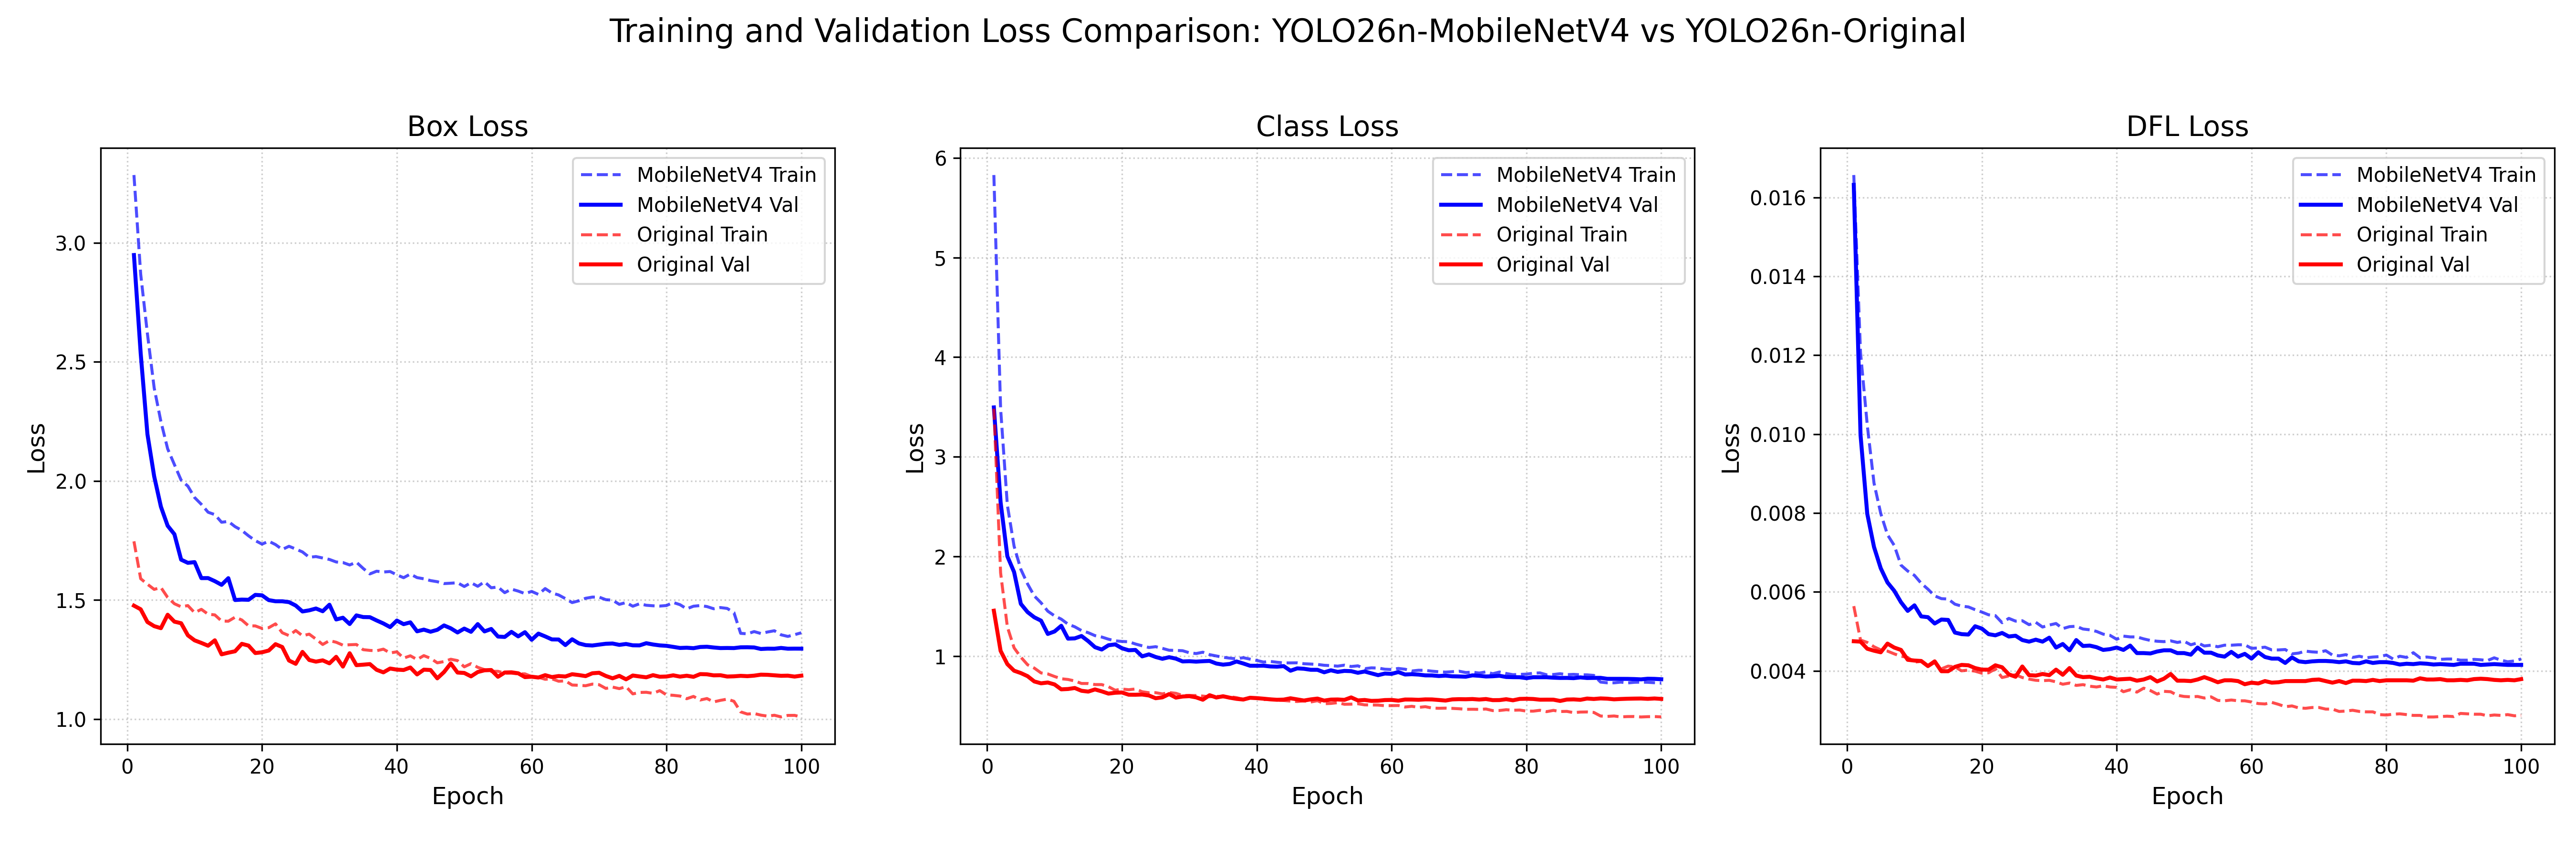
\includegraphics[width=\textwidth]{Images/chap3/loss_comparison.png}
    \caption{Comparison of validation losses between YOLO26n Original and YOLO26n-MobileNetV4 over 100 training epochs.}
    \label{fig:loss_comparison}
\end{figure}

Importantly, neither model shows signs of overfitting. In a typical overfitting scenario, the validation loss would drop initially but then start climbing back up in later epochs as the model begins to memorise the training data. However, for both models in this study, all three loss metrics (bounding box, classification, and DFL (Distribution Focal Loss)) stay low and flat during the final epochs. This confirms that they generalise well to unseen data.

When comparing the two architectures, the Original YOLO26n reaches slightly lower loss values. For example, its minimum bounding box loss drops to 1.1676, while the MobileNetV4 version stops at 1.2949. A similar pattern is seen in the classification loss (0.5529 vs 0.7694). This difference is entirely expected. Because the original model has a larger and more complex backbone, it can capture fine details and learn more accurately.

Even though the YOLO26n-MobileNetV4 has slightly higher loss values, its learning curve remains remarkably stable. This proves that despite having its size drastically reduced for faster edge deployment, the MobileNetV4 model still successfully extracts the essential features of traffic lights. It does not suffer from gradient issues or training instability. Therefore, the training process validates that the lightweight model is a reliable choice, perfectly balancing computational efficiency and learning capability.

\subsubsection{Architectural Decision Justification}

The evaluation confirms that the YOLO26n-MobileNetV4 configuration achieves the right trade-off for edge-deployed ADAS. Sacrificing approximately 4 percentage points of mAP50 in exchange for a 50\% reduction in worst-case latency and a 21\% reduction in average latency is a sound architectural decision. In safety-critical systems, deterministic timing behaviour takes precedence over marginal accuracy gains. The 85.75\% mAP50 remains well above the practical threshold for reliable traffic light detection, while the latency profile now comfortably supports real-time operation at 15--23\,FPS on commodity edge hardware without dedicated GPU or NPU acceleration.

